\section{Versuchsziel}
Die Bestimmung der Austrittsarbeit der Elektronen für das Metall Wolfram
unter Verwendung des glühelektrischen Effekts. Zudem soll die Kennlinie einer
Hochvakuumdiode bestimmt werden, in welcher der glühelektrische Effekt untersucht
werden kann.
\section{Theorie}
\label{sec:Theorie}
\paragraph{Potentialtopf}

Ein Elektron im Atomgitter des Metalls befindet sich, in grober Nährung,
in einem konstanten einheitlichen Potential. Das Potential außerhalb des Metalls
ist um den Faktor $ \Phi$ größer, dieses Potentialtopfmodell ist in der Abbildung
\ref{fig:Pot} dargestellt. Um das Metall verlassen zukönnen muss ein
Elektron die Austrittsarbeit $\symup{e}_0 \cdot \xi$ leisten. Hier bei bezeichnet
$\symup{e_0}$ die Elementarladung.
\begin{figure}
  \centering
  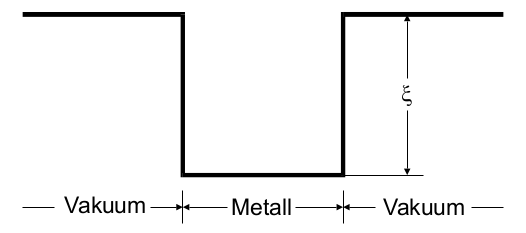
\includegraphics[height=3cm]{logos/Potentialtopf.png}
  \caption{Potentialtopf eines Metalles \cite{Anleitung}.}
  \label{fig:Pot}
\end{figure}
\FloatBarrier.
\paragraph{Fermi-Dirac Verteilung}
Die Fermi-Dirac Verteilung gibt die Wahrscheinlickeit an für die ein möglicher
Zustand mit der Energie $E$ im thermischen Gleichgewicht besetzt ist. Die
Fermi-Dirac-Funktion ist gegeben durch
\begin{equation}
  f\left(E\right) = \frac{1}{\exp\left(\frac{E - \zeta }{\symup{k_B}T+1}\right)}
\end{equation}
gegeben, dabei bezeichnet $T$ die Temperatur, $k_B$ die Boltzmann-Konstante und
$\zeta$ die Fermische Grenzenergie. Die Funktion ist in der Abbildung \ref{fig:FD}
dargestellt. Um aus der Metalloberfläche auszutretten müssen die Elektronen eine
Energie von $\zeta + e_0 \cdot \Phi$ besitze, da diese Energiewerte auch im
Schmelzpunkt von Wolfram noch groß im vergleich zu $k_B T $ sind kann die Närung
\begin{equation}
  f\left(E\right)= \exp\left(\frac{\zeta - E}{\symup{k_B} T} \right)
\end{equation}
benutzt werden.
\begin{figure}
  \centering
  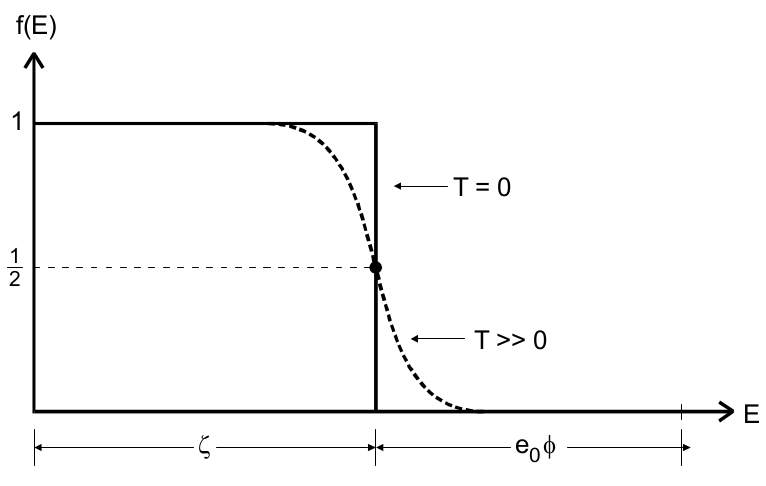
\includegraphics[height=5cm]{logos/Fermi-Dirac.png}
  \caption{Fermi-Dirac Verteilung am absoluten Nullpunkt
  \texorpdfstring{$T = 0$}{math} und \texorpdfstring{$T >> 0$}{math}
  \cite{Anleitung}.}
  \label{fig:FD}
\end{figure}
\FloatBarrier
\paragraph{Settigungsstromdichte}
Nun wird die Verteilungsfunktion von zuvor genommen und über alle Energien
integriert, bis auf die Energien in z-Richtung (also in Richtung Anode) größer als
$\zeta + e_0 \Phi$ liegen, diese werden von $\zeta + e_0 \Phi$ bis $infty$
integriert. Daraus folgt die Gleichung
\begin{equation}
  j_S(T) = 4\pi \frac{\symup{e_0} m_0 \symup{k_B} ^2 }{\symup{h^3}} T^2 \exp \left( \frac{-\symup{e_0} \Phi}{\symup{k_B} T}\right)\; ,
\end{equation}
diese Gleichung gibt die Sättigungsstromdichte die angibt wieviele Elektronen
die Metalloberfläche in Abhängigkeit von der Temperatur verlassen. Die Gleichung
wird auch als \textit{Richardson-Gleichung} bezeichnet. Hier bei bezeichnet
$m_0$ die Elektronenmasse und $h$ das Planchsche Wirkungsquantum.


\paragraph{Hochvakuum-Diode}
Eine Hochvakuum-Diode ist im Prinzip eine Kathode und Anode
eingelassen in einen Glaskörper in dem ein Hochvakuum herrscht. Die Anode saugt
die Elektronen die aus der Kathode austretten auf. Eine schematische Abbildung
ist in den Abbildungen \ref{fig:SDL} und \ref{fig:SAK} zu sehen.

\paragraph{Langmuir-Schottkysche Raumladungsgleichung}
Da die Geschwindigkeit der Elektronen die aus dem Metall austretten nicht
konstant ist folgt, dass die Raumladungsdichte $\rho$ in Richtung der Anode
abnimmt und damit die Kathode abschirmt. Der erwartete Diodenstrom ist als
kleiner als von der \textit{Richardson-Gleichung} erwartet. Ein Zusammenhang
zwischen der Anodenspannug und Diodenstrom lässt sich im Raumladungsbereich
über die \textit{Poisson Gleichung} konstruieren, dieser ist gegeben durch
\begin{equation}
  j = \frac{4}{9} \symup{\epsilon_0} \sqrt{\frac{2\symup{e_{0}}}{m_{0}}} \frac{V^{\frac{3}{2}}}{a^2} \,.
\end{equation}
Dabei bezeichnet $a$ den Abstand ziwschen der Kathode und Anode, $V$ ist das
Potential am Aufpunkt und $\symup{\epsilon_0}$ die Dielektrizitätskonstante des Vakuums.

\paragraph{Anlaufgebiet einer Hochvakuumdiode}
Wie schon zuvor besprochen gibt es endlich viele Elektronen die für $T > 0$ eine
Energie besitzen die größer ist als die Austrittsarbeit. Das hat zur Folge, dass
es Elektronen gibt, die bei einem schwachen Gegenfeld einen Anlaufstrom hervorrufen.
Ein solches Elektron besitzt die Energie $ \symup{e_0 }\Phi_A + \symup{e_0 }V$, dabei bezeichnet
$\Phi_A$ die Austrittsarbeit des Anodenmaterials und $V$ das von außen
angelegte Potential. Daraus ergibt sich dann
\begin{equation}
  j(V) = j_0 \exp \left(-\frac{\symup{e_0} \Phi_A + \symup{e_0} V}{\symup{k_B} T} \right) \;.
\end{equation}
\paragraph{Kennlinie der Hockvakuum-Diode}
Die Kennline der Hochvakuum-Diode zeigt den Zusammenhang zwischen
dem Anodenstrom $I$ und damit der Stromdichte $j$ und der Spannung $U$ also dem
angelegtem Potential. Wie in der Darstellung \ref{fig:KL} zusehen ist, kann die
Kennlinie in drei Bereiche eingeteilt werden. Zuerst das Anlaufstromgebiet
für $ V < 0$ in dem ein expotentieller Anstieg zu erkennen ist. Darauf folgt
das Raumladungsgebiet, in dem ein $\sqrt{V^3}$ Verlauf zu beobachten ist. Danach
kommt das Sätigungsstromgebiet. In dem sich der Strom asymptotisch einem
Sättigungsstrom annährt. Den Bezeichungen der Gebiete ist zu entnehmen, welche
oben genannten Gleichungen dort ihren Gültigkeitsbereich finden.
\begin{figure}
  \centering
  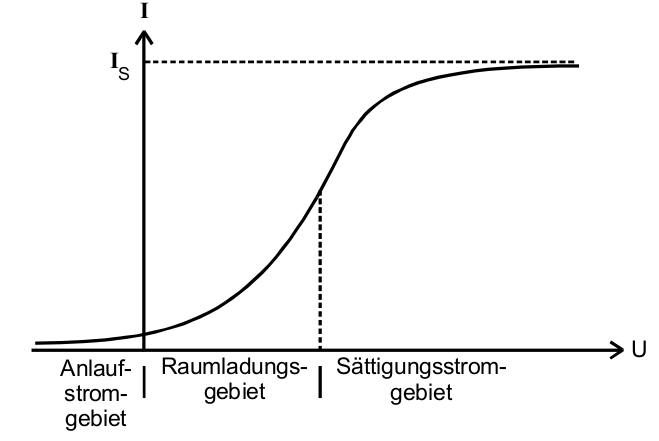
\includegraphics[height=5cm]{logos/Kennlinie.png}
  \caption{Kennlinie einer Hochvakkumdiode \cite{Anleitung}.}
  \label{fig:KL}
\end{figure}
